\documentclass[conference]{IEEEtran}
\IEEEoverridecommandlockouts
% The preceding line is only needed to identify funding in the first footnote. If that is unneeded, please comment it out.
\usepackage{cite}
\usepackage{amsmath,amssymb,amsfonts}
\usepackage{algorithm, algorithmic}
\usepackage{graphicx}
\usepackage{textcomp}
\usepackage{xcolor}
\def\BibTeX{{\rm B\kern-.05em{\sc i\kern-.025em b}\kern-.08em
    T\kern-.1667em\lower.7ex\hbox{E}\kern-.125emX}}
    
\newtheorem{definition}{Definition}
\usepackage{array}
\renewcommand{\arraystretch}{1.5}
\newcolumntype{L}[1]{>{\raggedright\let\newline\\\arraybackslash\hspace{2pt}}m{#1}}
\newcolumntype{C}[1]{>{\centering\let\newline\\\arraybackslash\hspace{2pt}}m{#1}}
\newcolumntype{R}[1]{>{\raggedleft\let\newline\\\arraybackslash\hspace{2pt}}m{#1}}

\def\correspondingauthor{\footnote{Corresponding author.}}

\begin{document}
\title{A Resource Usage Prediction System Using Functional-link and Genetic Algorithm Neural Network for Multivariate Cloud Metrics}
%{\footnotesize \textsuperscript{*}Note: Sub-titles are not captured in Xplore and
%should not be used}
%\thanks{Identify applicable funding agency here. If none, delete this.}

\author{
\IEEEauthorblockN{Thieu Nguyen, Nhuan Tran, Binh Minh Nguyen\IEEEauthorrefmark{1}\thanks{\IEEEauthorrefmark{1}Corresponding author.}}
\IEEEauthorblockA{\textit{School of Information and Communication Technology} \\
\textit{Hanoi University of Science and Technology}\\
Hanoi, Vietnam \\
nguyenthieu2102@gmail.com, tranducnhuan1994@gmail.com,\\\IEEEauthorrefmark{1}minhnb@soict.hust.edu.vn}
%\and
%\IEEEauthorblockN{Nhuan Tran}
%\IEEEauthorblockA{\textit{School of Information and Communication Technology} \\
%\textit{ Hanoi University of Science and Technology}\\
%Hanoi, Vietnam \\
%tranducnhuan1994@gmail.com}
%\and
%\IEEEauthorblockN{Binh Minh Nguyen\IEEEauthorrefmark{1}\thanks{\IEEEauthorrefmark{1}Corresponding author.}}
%\IEEEauthorblockA{\textit{School of Information and Communication Technology} \\
%\textit{ Hanoi University of Science and Technology}\\
%Hanoi, Vietnam \\
%minhnb@soict.hust.edu.vn}
\and
\IEEEauthorblockN{Giang Nguyen}
\IEEEauthorblockA{\textit{Institute of Informatics}\\
\textit{Slovak Academy of Sciences}\\
Bratislava, Slovakia \\
giang.ui@savba.sk}
}

\maketitle

\begin{abstract}
Designing prediction-based auto-scaling systems for cloud computing is an attractive topic for scientists today. However, there are many barriers, which must be solved before applying these systems to practice. Some challenges include: improving accuracy for prediction models, finding a simple and effective forecast method instead of complex techniques, and processing multivariate resource metrics at the same time. So far, there are no existing proactive auto-scaling solutions for clouds that have addressed all those challenges. In this paper, we present a novel cloud resource usage prediction system using functional-link neural network (FLNN). We propose an improvement for the FLNN by exploiting genetic algorithm (GA) to train learning model in order to increase forecast effectiveness. To deal with multivariate input data, several mechanisms also are combined together to enable the ability of processing simultaneously different resource types in our system. This enables to discover implicit relationship among diverse metrics and based on that realistic scaling decisions can be made closer to reality. We use Google trace dataset to evaluate the proposed prediction system and data preprocessing mechanisms introduced in this work. The gained outcomes demonstrated that our system can work effectively under practical situations with good performance as compared with traditional techniques.
\end{abstract}

\begin{IEEEkeywords}
Cloud computing, Functional-link neural network, Functional-link and Genetic algorithm neural network, FL-GANN, Proactive auto-scaling, Multivariate time series data, Genetic algorithm, Google trace dataset.
\end{IEEEkeywords}

\section{Introduction}
\label{intro}
Pay-as-you-go fashion is one of the prominent advantage features of cloud computing. With the usage model, users always expect their applications, which operate on cloud infrastructures are provided computational resources adequately but not redundantly in real-time without any delays. This helps reduce maximally the renting resource costs. However, it is quite difficult and complicated to meet the requirement because clouds must have a new scaling mechanism that can be tuned immediately and precisely offered resources on demand of these appliances to replace the current approach with resource usage thresholds. 

Indeed, although the setting threshold mechanism enables to define scaling rules easily, it cannot supply accurately resources as compared with the changeful requirements of applications. For example, assuming CPU percentage threshold of virtual machine (VM) is set at 80\% to scale out. When CPU utilization reaches the threshold, cloud will automatically add one more VM for the user’s system. However, the scaling function needs to spend a few moments to complete the deployment of second VM. During this time, the CPU percentage usage has already been changed from the set threshold to another that can be bigger or smaller than 80\%. This makes the inaccuracy issue for current cloud auto-scalers as presented above.

Besides, due to quality of service (QoS) tie with users (which is defined in service-layer agreements - SLA), cloud vendors often accept the resource over-provisioning (despite sometime the cloud users cannot acquire enough resources like) rather than offering resource accurately in real-time. This leads to the increase of infrastructure costs in general for both cloud users and providers. It can be seen that there is a long distance among the resource supply requirements of users and the vendors' capabilities with the cloud auto-scaling solution today. Hence, proposing a better auto-scaler to resolve the problem has significant for cloud computing adoption at this time.  

Recently, many prediction-based auto-scaling systems have been proposed for cloud computing. While increasing prediction accuracy for resource consumptions is a very attractive challenge, the problem of processing multiple metric types (e.g. CPU, and memory usages, disk capacity and I/O, network throughput/throughout and so forth) at the same time have received less attention from researchers when they develop prediction systems. Among the resource metrics could have some implicit relationships (e.g. between CPU and memory usage, and between disk I/O and memory I/O) and forecasting separately each resource type cannot discover the relationships. In this way, prediction outcomes will not fit practice requirements. To resolve the issue, cloud prediction-based auto-scalers has to the ability of processing different metrics simultaneously to make the scaling decision precisely. Until now, there are very few studies dealt with that multivariate problem for clouds. In this paper, we focus on proposing a new method for prediction stage using functional-link neural network (FLNN) and genetic algorithm (GA). Our forecast system also is designed to process multiple resource metrics simultaneously. We use real dataset produced from Google cluster to test and evaluate our designed model. The gained results show that our proposals bring positive effectiveness in predicting resource consumption.

The organization of this paper is as follows. In Section~\ref{related_work}, we categorize and analyze existing works to highlight our contributions. Section~\ref{fl_gann} presents our design cloud resource consumption prediction system with FN-GANN - an improvement of traditional FLNN using genetic algorithm to train model. We also introduce several proposed data preprocessing mechanisms in this section. In the next Section, we describe our tests, evaluations for the proposed system to prove the proposal effectiveness. Section~\ref{conclusion} concludes this paper and defines some our future works.

\begin{figure*}[h]
	\centerline{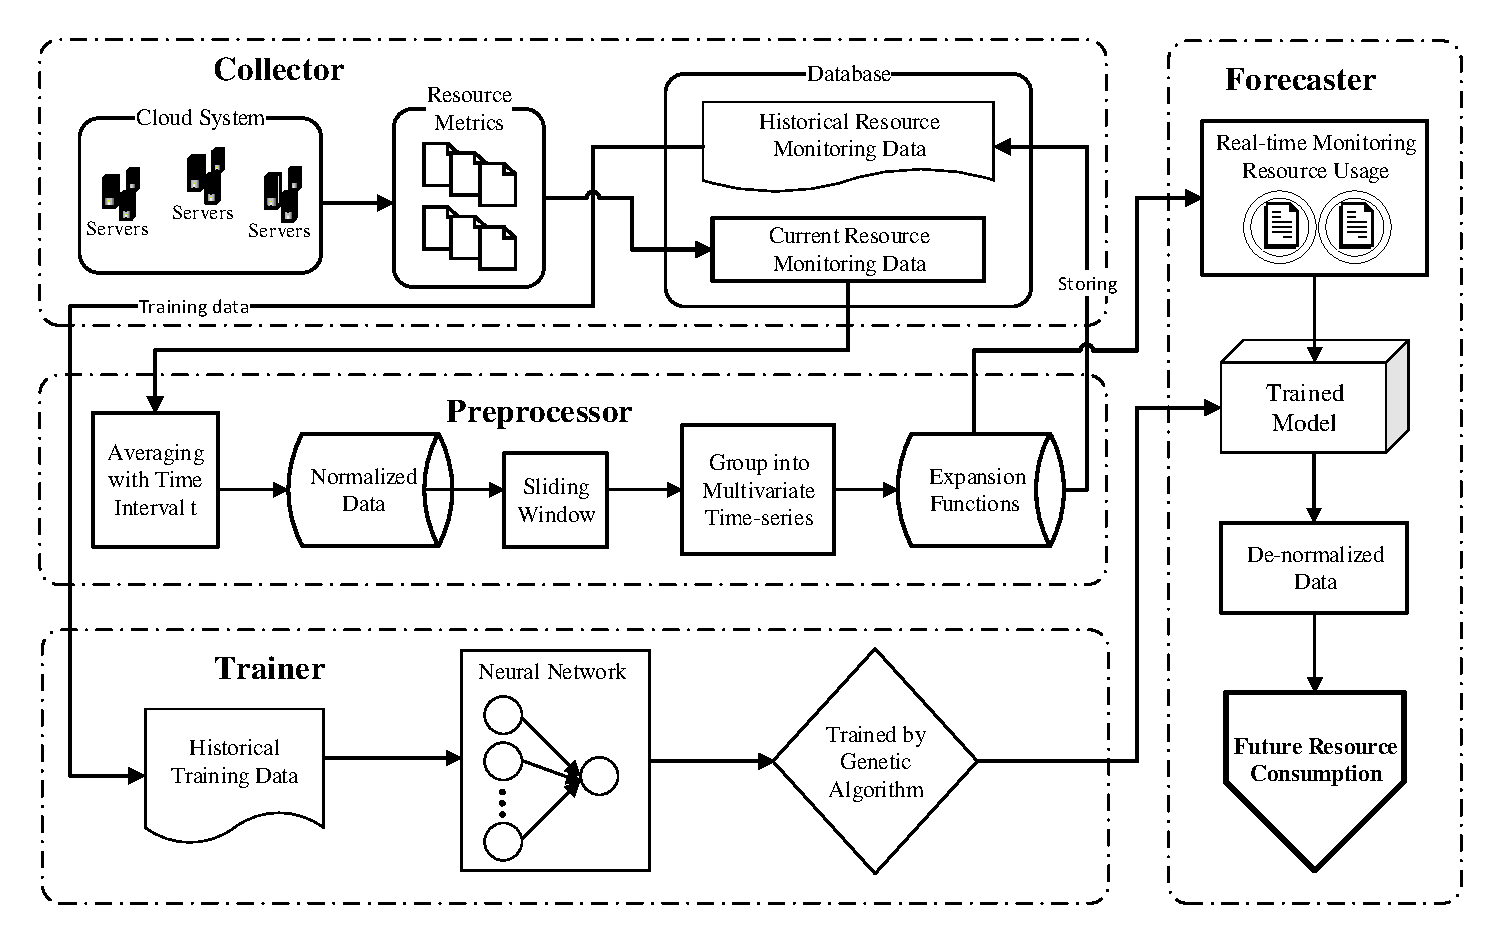
\includegraphics[width=0.7\textwidth =0.1cm 0.1cm 0.1cm 0.1cm, clip]{images/FLGANN_system.pdf}}
	\caption{Multivariate Resources Forecasting System}
	\label{FLGANN_system}
\end{figure*}
     
\section{Related Work}
\label{related_work}

The main goal of proactive resource provision techniques is to predict precisely the resource consumptions in advance. There are a huge research number that have dealt in forecast models for cloud computing. In [14], several models of predictive time series are
proposed and demonstrated such as ARMA (autoregressive-moving average),
nonstationary, long memory, three families of seasonal, multiple input-output,
intervention and multivariate ARMA models for predicting cloud workloads.

In~\cite{ref_hipel}, several prediction methods including autoregressive (AR), moving average (MA), autoregressive-moving average (ARMA), nonstationary, long memory, three families of seasonal, multiple input-output, intervention and multivariate ARMA models were evaluated and compared in predicting cloud workloads. 

Recently, deep learning has emerged as an effective solution for prediction problem. In terms of applying to clouds, Prevost et al.~\cite{ref_prevost} used the Multi-layer neural network (MLNN) model for prediction URL resource requests of a WWW server at NASA and WWW server at EPA. Although deep learning brings significant effectiveness for the cloud proactive auto-scaling issue, these learning models often have very complex structure and require a long time for training process. In this way, few other artificial networks have been proposed to overcome the disadvantages. Functional Link Neural Network is a representation for that simple neural network group.

FLNN has a single neuron is proposed by Pao~\cite{ref_pao} in pattern-recognition task. The author pointed out that FLNN has less computational cost and can be easily implemented in hardware applications. The reason is that hidden layer in this network is eliminated. In this way, nonlinear relationship between the inputs and outputs is processed via a set of functional expansions (i.e. polynomials). FLNN has been used in several applications such as stock market~\cite{ref_majhi}, and exchange rate prediction~\cite{ref_rout}. In their work, Khandelwal et al.~\cite{ref_khan} used 4 datasets from 4 different areas to test the forecasting ability of FLNN and in comparison with MLNN, the authors' obtained results indicate that FLNN model provides better outcomes for all 4 datasets. In~\cite{ref_sahoo}, Sahoo et al used efficient Chebyshev and Legendre polynomials in combination as Functional-Link, the FLNN's outcomes gives better accuracy and takes less computation time as compared to MLNN's outcomes.

However, the proposed prediction systems using FLNN listed above which still use back-propagation technique with gradients descent to train learning model. S. Dehuri at el. in~\cite{ref_dehuri} figured out that the main drawbacks of back-propagation are slow training speed and local minimum traps. In comparison with those existing works, the main difference given in this study is that we exploit a herd evolution algorithm to solve back propagation disadvantages in traditional FLNN. 

Genetic algorithm is one of optimization mechanisms for large and complex spaces in order to find values, which are close to the global optimum. Hence, GA suits the problem of training feed-forward networks~\cite{ref_motana}. In this direction, applying GA to diverse neural network variants have been proposed long time ago. In~\cite{ref_blanco}, Blanco et al. used GA-based approach to selected the features and optimized the appropriate classifier parameters of neural network and vector machines for bearing fault detection from time-domain vibration signals. In their work~\cite{ref_dehuri_2}, Dehuri et al. employed GA to choose an optimal subset of input features in FLNN and radial basis function neural network (RBFNN). Until now, there are no works, which use GA to train FLNN instead of back-propagation algorithm. 

In the aspect of dealing with multivariate time series problem in cloud computing, in~\cite{ref_dang}, the authors proposed MF-GABPNN model to mine the relationship among different metric types in forecast process. Thus, the authors choose CPU and memory as multivariate time-series to test their proposed model. Going further, in~\cite{ref_nhuan}, Nhuan et al. proved that there is a relation among different metric types and through analyzing data correlation, the authors select appropriate time series data metrics to put into LSTM-RNN prediction model. However, so far, there are no any studies that use FLNN for multivariate time series data prediction for cloud computing. As compared with the existing works presented above, our differences and contributions include:

\begin{enumerate}
	\item Proposing an new approach for proactive auto-scaling problem in clouds using FLNN.
	\item Proposing a novel improvement for FLNN, in which the network is trained by GA instead of back-propagation mechanism called FL-GANN. 
	\item Proposing a prediction resource forecasting system that can be processed multivariate data. This is an important feature of cloud computing while designing auto-scalers in practice.
	\item Testing the proposed system performance with real dataset produced by Google cluster.
\end{enumerate}

\section{Functional-Link Generic Algorithm Neural Network}
\label{fl_gann}
\subsection{Designing Prediction System}
\label{designing_system}

Our designs for cloud resources forecasting system are shown by figure~\ref{FLGANN_system} with four main modules, including Collector, Preprocessor, Trainer, and Forecaster.

Through Collector module, raw resource monitoring data is collected from VMs and stored in a repository. Currently, there are a lot of available monitoring services for public clouds such as CloudWatch of Amazon Web Services, IBM cloud monitoring, and Rackspace Monitoring and so forth. In addition, users can deploy and configure monitoring tools like Nagios, Prometheus and Zabbix by themselves on their VMs. The database in this module is used to store current resources monitoring data, which is produced in form of time-series and historical resources monitoring data, which is made by Preprocessor module. 

Preprocessor module plays the role of transforming the collected raw time-series data to supervised data to fit the input of neural network. There are several mechanisms that are deployed to process cloud workload data, covering: averaging data in long time period, normalized data, sliding window, group into multivariate time series and expansion functions. After preprocessing in this module, the output data is put into database in Collector as historical resources data, which is used to create prediction model in Trainer module. The data also is provided for Forecaster to predict consumption resources. 

A novel learning method is proposed in our Trainer module using FLNN that is a variant of traditional neural network using expansion functions. Furthermore, the network also is trained by GA to speed up the convergence and increase the forecast accuracy. Due to combination of those mechanisms, the proposed learning method is called by FL-GANN. 

After the training process finishes, trained model is used to predict future resource consumption in Forecaster. 

\begin{figure*}[htbp]
	\centerline{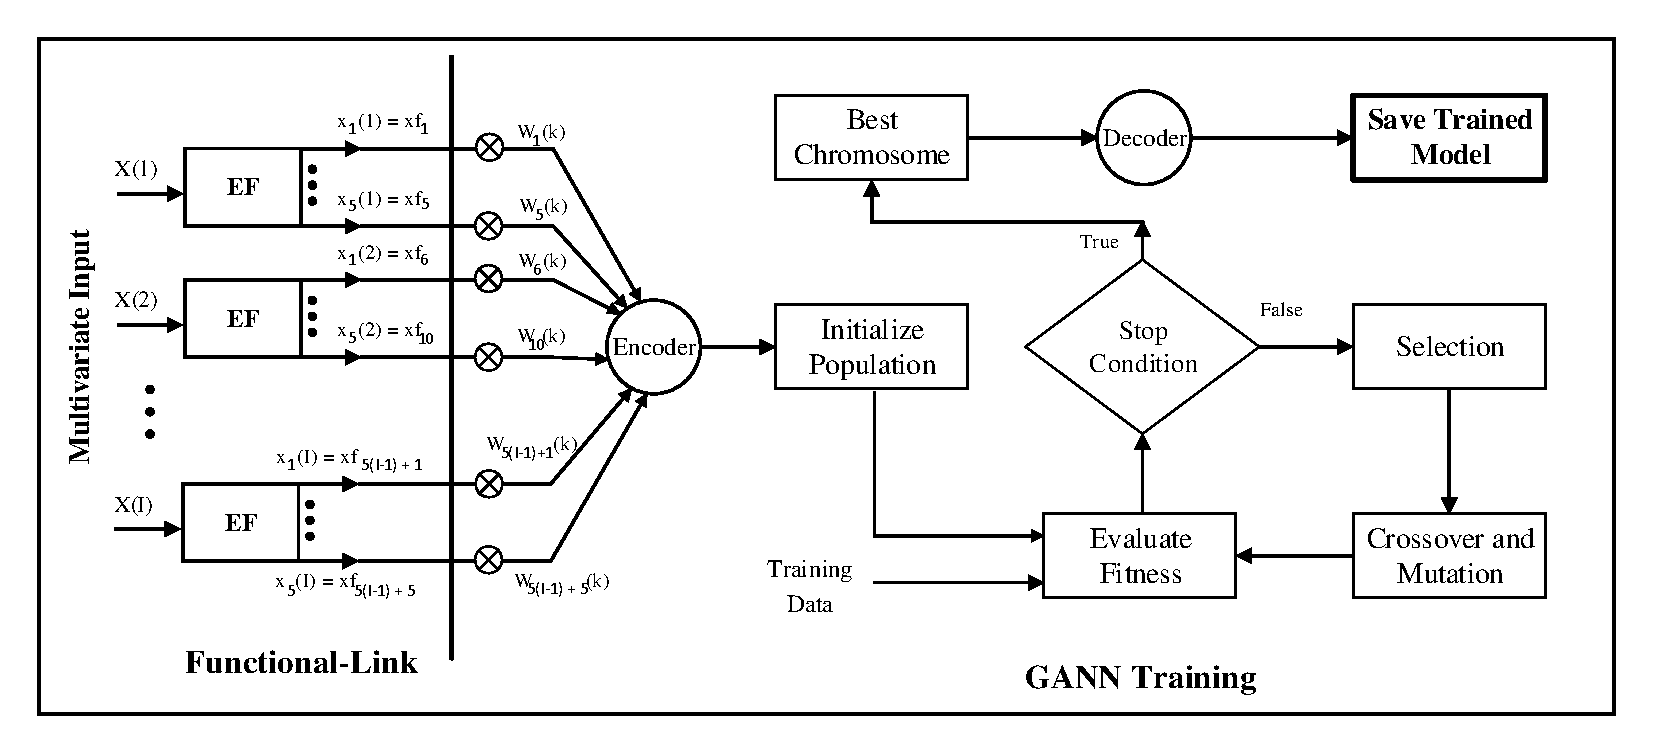
\includegraphics[width=0.7\textwidth =0.1cm 0.1cm 0.1cm 0.1cm, clip]{images/FLGANN_process.pdf}}
	\caption{FL-GANN training process}
	\label{FLGANN_process}
\end{figure*}

\subsection{Preprocessing Monitoring Data}
\label{pre_precessor}

As presented before, the goal of Preprocessor is to prepare data for Trainer and Forecaster. There are five mechanisms deployed in this component. Firstly, the current raw data gathered in a long period is transformed into the corresponding time series $r_i(t) (i = 1, 2,..., M)$ with time interval $\rho$. Each point in time series $r_i(t)$ is calculated by averaging all the values of a resource metric usage in the period of $\rho$ as follows: $r_i(n) = \frac{ \sum_{i=(n-1)\rho < t < n\rho}^nD_i(t) }{ n_{\rho} }$, where $D_i(t)$ is the value of type-i resource at time $t$ that is monitored from cloud system, $n\rho$ is the number of observation $D_i(t)$ in the interval $\rho$. 

The next phase is normalization, which scales a time series in the range of [0, 1]. Then, time-series data is transformed to supervised data by using sliding method with window width $k$ that is the number of values before time $t$ to predict value at the time $t$. Then all resource metric types are grouped into single multivariate data. Finally, the gained multivariate data undergoes expansion functions such as Chebyshev, Legendre or Power to enable the ability of catching the nonlinear relationship between the inputs and outputs for our neural network. The reason is there are no a hidden layers in the network architecture. Concept of multivariate time series is defined by Definition~\ref{definition_1}. Meanwhile, functions link that is used in expansion functions component is introduced by Definition~\ref{definition_2}.

\begin{definition}
\label{definition_1}
Let $X_1(t), X_2(t),. . . , X_i(t),. . . , X_M(t) $ are $M$ time series ($M$ metrics resource types), the single multivariate time series is: \\
$ X(t) = \left[ X_1(t), X_2(t), . . . , X_M (t) \right],  t = 1, 2, . . . , n$.
\end{definition}

\begin{definition}
\label{definition_2}
A functional link is a function $f$ $\in$ $R^D \rightarrow R$ that transforms $X$ to a scalar ($X$: vector input patterns). If the input layer of the FLNN consists of functional link $f_i$, $i = 1,2,..., n$ then input patterns $X$ will be transformed to $Y$ $\in R^n$: $Y = (f_1(X),... f_n(X))$. 
\end{definition}

There are many expansion functions, however the most popular are Chebyshev, Legendre, Laguerre, Power Series, Trigonometric. 

\subsection{Trainer module}
\label{learning_model}
This module consists of two main components, covering a neural network with single unit and GA, which is used to train the network. The functional link of FLNN are deployed in Preprocessor as presented in Subsection~\ref{pre_precessor}. Figure~\ref{FLGANN_process} describes general training process of our proposed FL-GANN model. In Fig.~\ref{FLGANN_process}, there is a component Encoder, which real-value encodes the weights and bias of network into a chromosome (real-value vector), while the Decoder component decoded the chromosome into the weights and bias of network. Because the requirement of GA is a fitness function, we calculate Mean Absolute Error (MAE) based on error of training data according to formula (\ref{eq_MAE}). The fitness function is reckoned by equation (\ref{eq_fitness}). Operations of GA in FL-GANN model are introduced via Algorithm~\ref{algo_GA}.

\begin{algorithm}[h]
	\caption{GANN Training Algorithm}\label{algo_GA}
	\hspace*{\algorithmicindent} \textbf{Input:} 
	\textbf{ $p_s$ } - the population size \\
	\hspace*{\algorithmicindent} \textbf{$d$} - problem size / d-dimension vector of each individual,\\
	\hspace*{\algorithmicindent} \textbf{ $p_c$ } - the probability of 2 individual exchanging crossovers,\\
	\hspace*{\algorithmicindent} \textbf{$p_m$ } - the probability of individual mutation, \\
	\hspace*{\algorithmicindent} \textbf{$g_{max}$} - the maximum number of generations \\
	\hspace*{\algorithmicindent} \textbf{Output:} The best chromosome. 
	
	\begin{algorithmic}[1]
		\STATE Initializing population $P$ = $ \left\{ C_1,. . . , C_{p_s} \right\}$, each individual is a d-dimension vector $C_i = (c_{i1}, …, c_{id})$, $c_{ij} \in $ [-1, 1]
		\STATE g $\leftarrow$ 1 
		\WHILE{$g \le gmax$ } 
		\STATE Calculating fitness of population based on formula (2)
		\STATE Finding the best chromosome $C_{best}$ according to the achieved fitness value.
		\REPEAT 
		\STATE Using Routtele Wheel Selection to choose two individuals (parents $p_1, p_2$) based on the fitness value to cross-over with probability $p_c$ to make 2 offspring ($CH_1, CH_2$)  based on:
		\STATE 	$CH_{1i} \leftarrow \lambda p_{1i} + (1- \lambda)p_{2i}$
		\STATE	$CH_{2i} \leftarrow \lambda p_{2i} + (1- \lambda)p_{1i}$, 		$ \lambda \sim U(0,1), i = \overline{1, d} $
		\STATE Then offspring undergo  the mutation process by replacing each $CH_{ij}, i = \overline{1, 2}, j = \overline{1, d},$ with probability $p_m$ by a random uniform value $\sim U(0,1)$.
		\STATE Appending offspring into a new generation.
		\UNTIL{new generation has $p_s$ individuals}
		\STATE Replacing the old generation by the new generation. 
		\STATE g $\leftarrow$ $g + 1$
		\ENDWHILE
		\STATE Return $C_{best}$
	\end{algorithmic}
\end{algorithm}

\begin{equation} 
MAE = \frac{\sum_{i=0}^N( forecast(i) - y_i)^2}{N}	\label{eq_MAE}
\end{equation}

\begin{equation} 
Fitness = \frac{1}{MAE}	\label{eq_fitness}
\end{equation}

\subsection{Forecaster Module}
\label{forecater}
Our Forecaster module uses values of real-time monitoring data (after preprocessing process) as inputs of the trained model to predict new values (i.e. resource consumption) in advance. Before can be used, the obtained outputs are unnormalized into the real values.

\section{Experiments}
\label{experiments}

\begin{table*}[h]
	\caption{MAE comparison of MLNN, traditional FLNN and FL-GANN models}
	\begin{center}
		\begin{tabular}{| c | c| c | c | c | c | c | c |}
			\hline
			\textbf{Input Type} & \textbf{Model} & \multicolumn{3}{c}{\textbf{CPU}}  & \multicolumn{3}{|c|}{\textbf{RAM}}  \\ \cline{3-8} 
			& & k = 2 & k = 3 & k = 5 & k = 2 & k = 3 & k = 5  \\ [0.5ex] \hline
			& MLNN & 0.3327	& 0.3514 & 0.3570	& 0.0288	& 0.0265 	& 0.0273  \\ 
			Univariate & FLNN	& 0.2944 	& 0.2999  & 0.3054	& 0.0210 	& 0.0201 	& 0.0215  \\
			& FL-GANN	& \textbf{0.2829}	& \textbf{0.2812} & \textbf{0.2843}	& \textbf{0.0195} 	& \textbf{0.0197}	& \textbf{0.0202}  \\ \hline
			
			& MLNN	& 0.3314	& 0.3387 	& 0.3448	& 0.0266 & 0.0271	& 0.0289 \\ 
			Multivariate & FLNN	& 0.2971 	& 0.2903 	& 0.3201	 & 0.0218  & 0.0202	& 0.0226   \\ 
			& FL-GANN	& \textbf{0.2815}	& \textbf{0.2814} 	& \textbf{0.2902}	& \textbf{0.0194} & 0.0207	& \textbf{0.0212}   \\ \hline 
		\end{tabular}
		\label{table:forecasting_results_MLNN_FLNN_FLGANN}
	\end{center}
\end{table*}
In this section, we present experiments as well as evaluations for our proposed system. The tests cover: 
\begin{enumerate}
	\item Comparing prediction accuracy between MLNN, traditional FLNN and FL-GANN;
	\item Evaluating influence of GA hyper-parameters on FL-GANN performance;
	\item Evaluating influence of FLNN expansion functions on FL-GANN effectiveness. 
\end{enumerate}

\subsection{Experimental Setup}
\label{experimental_setup}

In our experiments, we use a real workload dataset provided by Google~\cite{ref_google_trace} in one month of 2011. In the dataset, each job is a collection of many tasks that are run simultaneously on multiple machines. Resource utilization of tasks are measured by several metrics such as CPU, and memory usage, disk I/O mean time, and so on. According to the analyses also presented in~\cite{ref_google_trace}, only less than 2$\%$ of jobs run for longer than one day, even though such jobs contribute to over 80$\%$ of the recorded resource utilization in the Google cluster. In order to evaluate the generalization of our prediction model, we select a long running job with ID 6176858948. The job consists of 60171 divergent tasks during the 20-day period (from 1st to 20th day). We set average time $t$ = 5 minutes, forecast horizon $k$ = 1 in all experiments. The data from 1st to 15th day is used to train neural networks. Meanwhile, the data from 16th to 20th day is employed to test the prediction performance of these networks. For the multivariate input case, both CPU and memory usage data is used simultaneously for the learning models. Meanwhile, in the case of univariate, only one metric (CPU or memory) is put into the prediction models. Because we do not want to repeat the comparison between the models in [14], so we mainly focus on networks including MLNN, traditional FLNN and our proposed model Functional-Link Genetic Algorithm Neural Network(FL-GANN).


\begin{figure*}[h]
	\centering
	\begin{minipage}[t]{8cm}
		\centering
		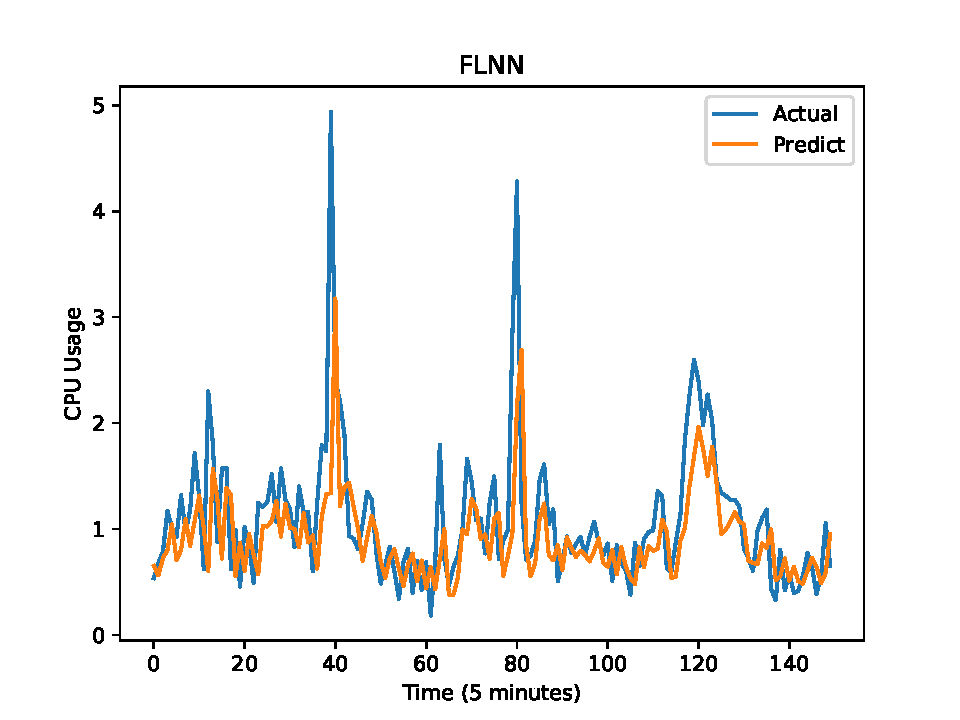
\includegraphics[width=0.8\textwidth =0.2cm 0.2cm 0.2cm 0.2cm]{images/multi_cpu_flnn.pdf}
	\end{minipage}
	\hspace{0.5cm}
	\begin{minipage}[t]{8cm}
		\centering
		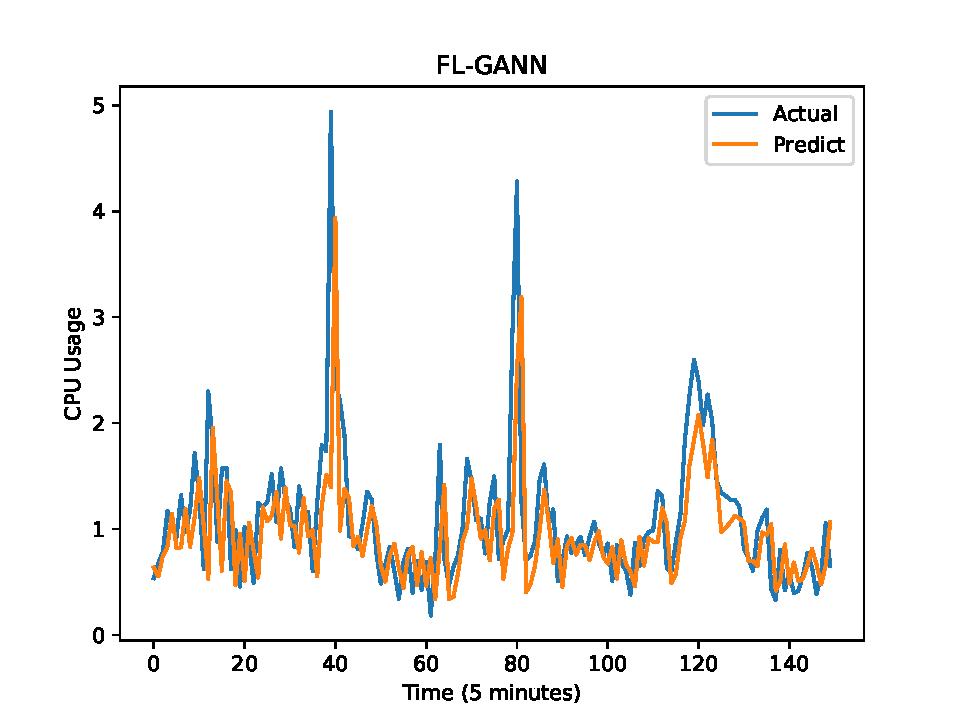
\includegraphics[width=0.8\textwidth =0.2cm 0.2cm 0.2cm 0.2cm]{images/multi_cpu_flgann.pdf}
	\end{minipage}
	\caption{CPU prediction outcomes of FLNN and FL-GANN with multivariate input data} 
	\label{tn1_multi_CPU}
\end{figure*}

\begin{figure*}[h]
	\centering
	\begin{minipage}[t]{8cm}
		\centering
		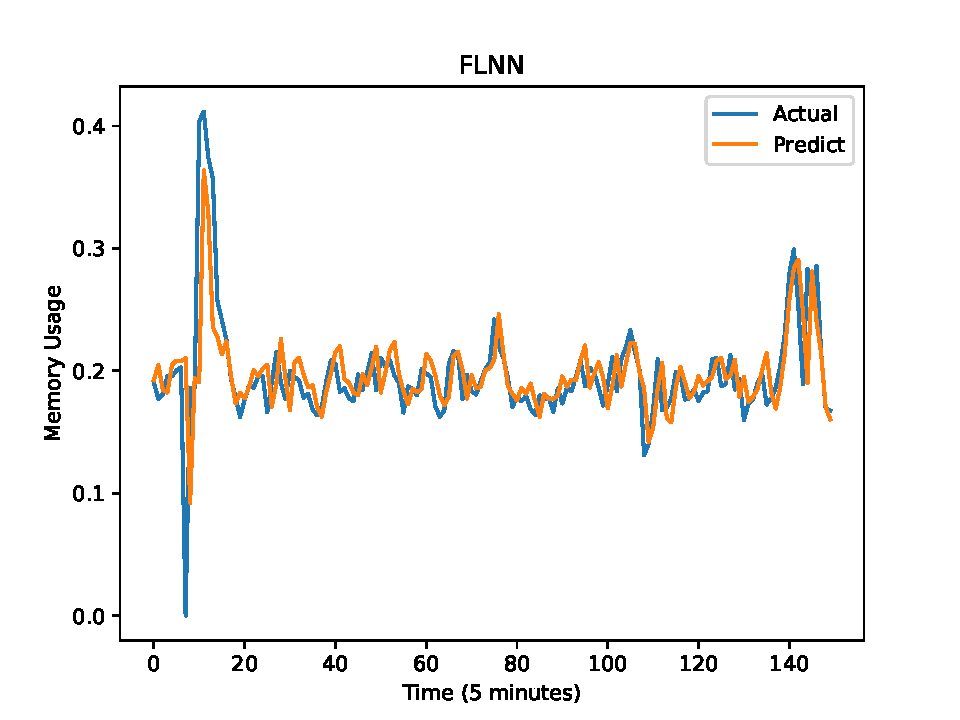
\includegraphics[width=0.8\textwidth =0.2cm 0.2cm 0.2cm 0.2cm]{images/multi_ram_flnn.pdf}
	\end{minipage}
	\hspace{0.5cm}
	\begin{minipage}[t]{8cm}
		\centering
		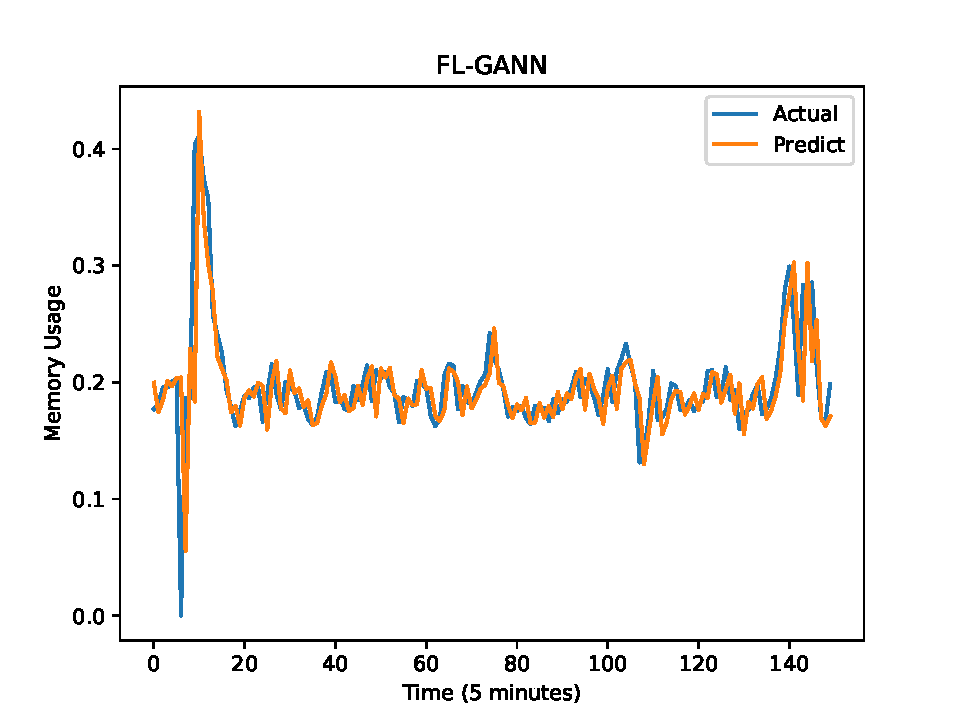
\includegraphics[width=0.8\textwidth =0.2cm 0.2cm 0.2cm 0.2cm]{images/multi_ram_flgann.pdf}
	\end{minipage}
	\caption{Memory prediction outcomes of FLNN and FL-GANN with multivariate input data} 
	\label{tn1_multi_RAM}
\end{figure*}

Our MLNN is configured with 5 layers (1 input, 1 output and 3 hidden). The neuron number for layers is set in succession as follows: $k$, 10, 15, 5, and 1. Traditional FLNN and FL-GANN have only one input and output layer with structure $(k, 1)$. Here, $k$ is the sliding window value used in the Preprocessor module. Activation function used for all three networks are Exponential Linear Unit (ELU). 

\subsection{Forecasting Resource Consumption with Multivariate Input Data}
\label{forecast}

In this test, we evaluate the efficiency of FL-GANN against MLNN, and traditional FLNN in forecasting resource consumption. For each model, we also compare univariate (single input metric) and multivariate (multiple input metrics) data. We change sliding windows size $k$ from 2 to 5 ($k$ = 2, 3, 5) in this test. Our achieved MAE outcomes are given in Table~\ref{table:forecasting_results_MLNN_FLNN_FLGANN}.

The results point out that MAE accuracy of FL-GANN are almost smaller than FLNN and MLNN model with different sliding window values as well as input types. Concretely, in the case of univariate data input, FL-GANN brings the best results in comparison with traditional FLNN and MLNN. For multivariate data, there is only one case of $k$ = 3 and memory consumption prediction, MAE of FL-GANN is lower than traditional FLNN. Otherwise, the FL-GANN has better performance as compared with other models.

Figure~\ref{tn1_multi_CPU} and~\ref{tn1_multi_RAM} show the predicted results between FLNN and FL-GANN models for CPU and memory with multivariate input data. While, the blue line is the actual usage, orange line is the predicted values. It can be seen that prediction curve of FL-GANN tends to closer to the actual value curve in comparison with forecast FLNN curve for both CPU and memory with multivariate input data. Also, for the weirdo points (both high and low), the results also show that the FL-GANN model is better than FLNN and MLNN.

\subsection{Influence of GA hyper-parameter on FL-GANN}
\label{influence1}
In this experiment, we focus on evaluating the influence of different GA hyper-parameters on our FL-GANN with multivariate input data. The parameters are pre-set for this test as follows.

\begin{enumerate}
	\item For population size $p_s$ changing experiment: $p_s$ value is put out in turn from $\left\{50, 100, 200, 300, 400, 500, 600\right\}$, sliding window = 3, expansion functions is Power Series, $g_{max} = 650$,  $p_c = 0.95$, and $p_m = 0.025$.	
	\item For probability of two individual exchanging crossover $p_c$ changing experiment: $p_c$ value is put out in turn from $\left\{ 0.70, 0.75, 0.80, 0.85, 0.90, 0.95, 0.98 \right\}$, sliding window = 3, expansion functions is Power Series, $g_{max} = 650$, $p_s = 500$, and $p_m = 0.025$.
	\item For probability of individual mutation $p_m$ changing experiment: $p_m$ value is put out in turn from $\left\{ 0.005, 0.01, 0.025, 0.05, 0.065, 0.80, 0.10 \right\}$, sliding window = 3, expansion functions is Power Series, $g_{max} = 650$, $p_s = 400$, and $p_c = 0.95$.
\end{enumerate}

\textbf{Population size changing experiment.} For each $p_s$, we carry on 20 times of MAE and RMSE measurements then calculate average values, which are shown in Table~\ref{table:2_population_size}. The evident observation is that with $p_s$ = 50, MAE's and RMSE's average values reach the biggest numbers at 0.2988, and 0.4913, respectively. When $p_s$ = 600, the both average error accuracy values are the smallest number at 0.2899, and 0.4821, respectively. Moreover, the MAE results are produced by $p_s$ at 400, and 500 that approximate the value is produced by $p_s$ at 600 although population size is increased by 100 and 200, respectively. Based on figure~\ref{tn2_CPU_ps_FLGANN}, we also recognize that MAE values of $p_s$ at 400, and 500 are smaller than MAE values of $p_s$ at 600. This infers that the smaller population, the worse of outcomes and if the population is large, the results may be better. However, in that case, the proposed model will take time to learn. Hence, the population size is from 300 to 600 producing acceptable performance for the tested data.

Figure~\ref{tn2_CPU_ps_FLGANN} indicates the MAE range of population sizes with diverse $p_s$ parameters using box-and-whisker plots. While the intermittent lines in the middle of boxes represent the mean values, the upper and lower boundaries of the boxes represents upper and lower quantiles of the distributions. Via those results shown by this figure, a remark could be brought forward as follow. The population size has the smallest average MAE accuracy at $p_s$ = 600 (average MAE is equal to 0.2898 in this case).

\begin{table}[h]
\caption{Comparison of average MAE with different population sizes} 
\begin{center}
\begin{tabular}{| c | c| c |}
\hline
\textbf{Population size} & \multicolumn{2}{c|}{\textbf{Error Accuracy}}  \\ \cline{2-3} 
& MAE & RMSE \\ [0.5ex] \hline
$p_s$ = 50	& 0.2988	& 0.4913 \\ \hline
$p_s$ = 100	& 0.2940	& 0.4846 \\ \hline
$p_s$ = 200	& 0.2925	& 0.4860 \\ \hline
$p_s$ = 300	& 0.2924	& 0.4833 \\ \hline
$p_s$ = 400	& 0.2907	& 0.4834 \\ \hline
$p_s$ = 500	& 0.2908	& 0.4823 \\ \hline
\textbf{$p_s$ = 600}	& \textbf{0.2899}	& \textbf{0.4821} \\ \hline
\end{tabular}
\label{table:2_population_size}
\end{center}
\end{table}

\begin{figure*}[h]
	\centering
	\begin{minipage}[t]{8cm}
		\centering
		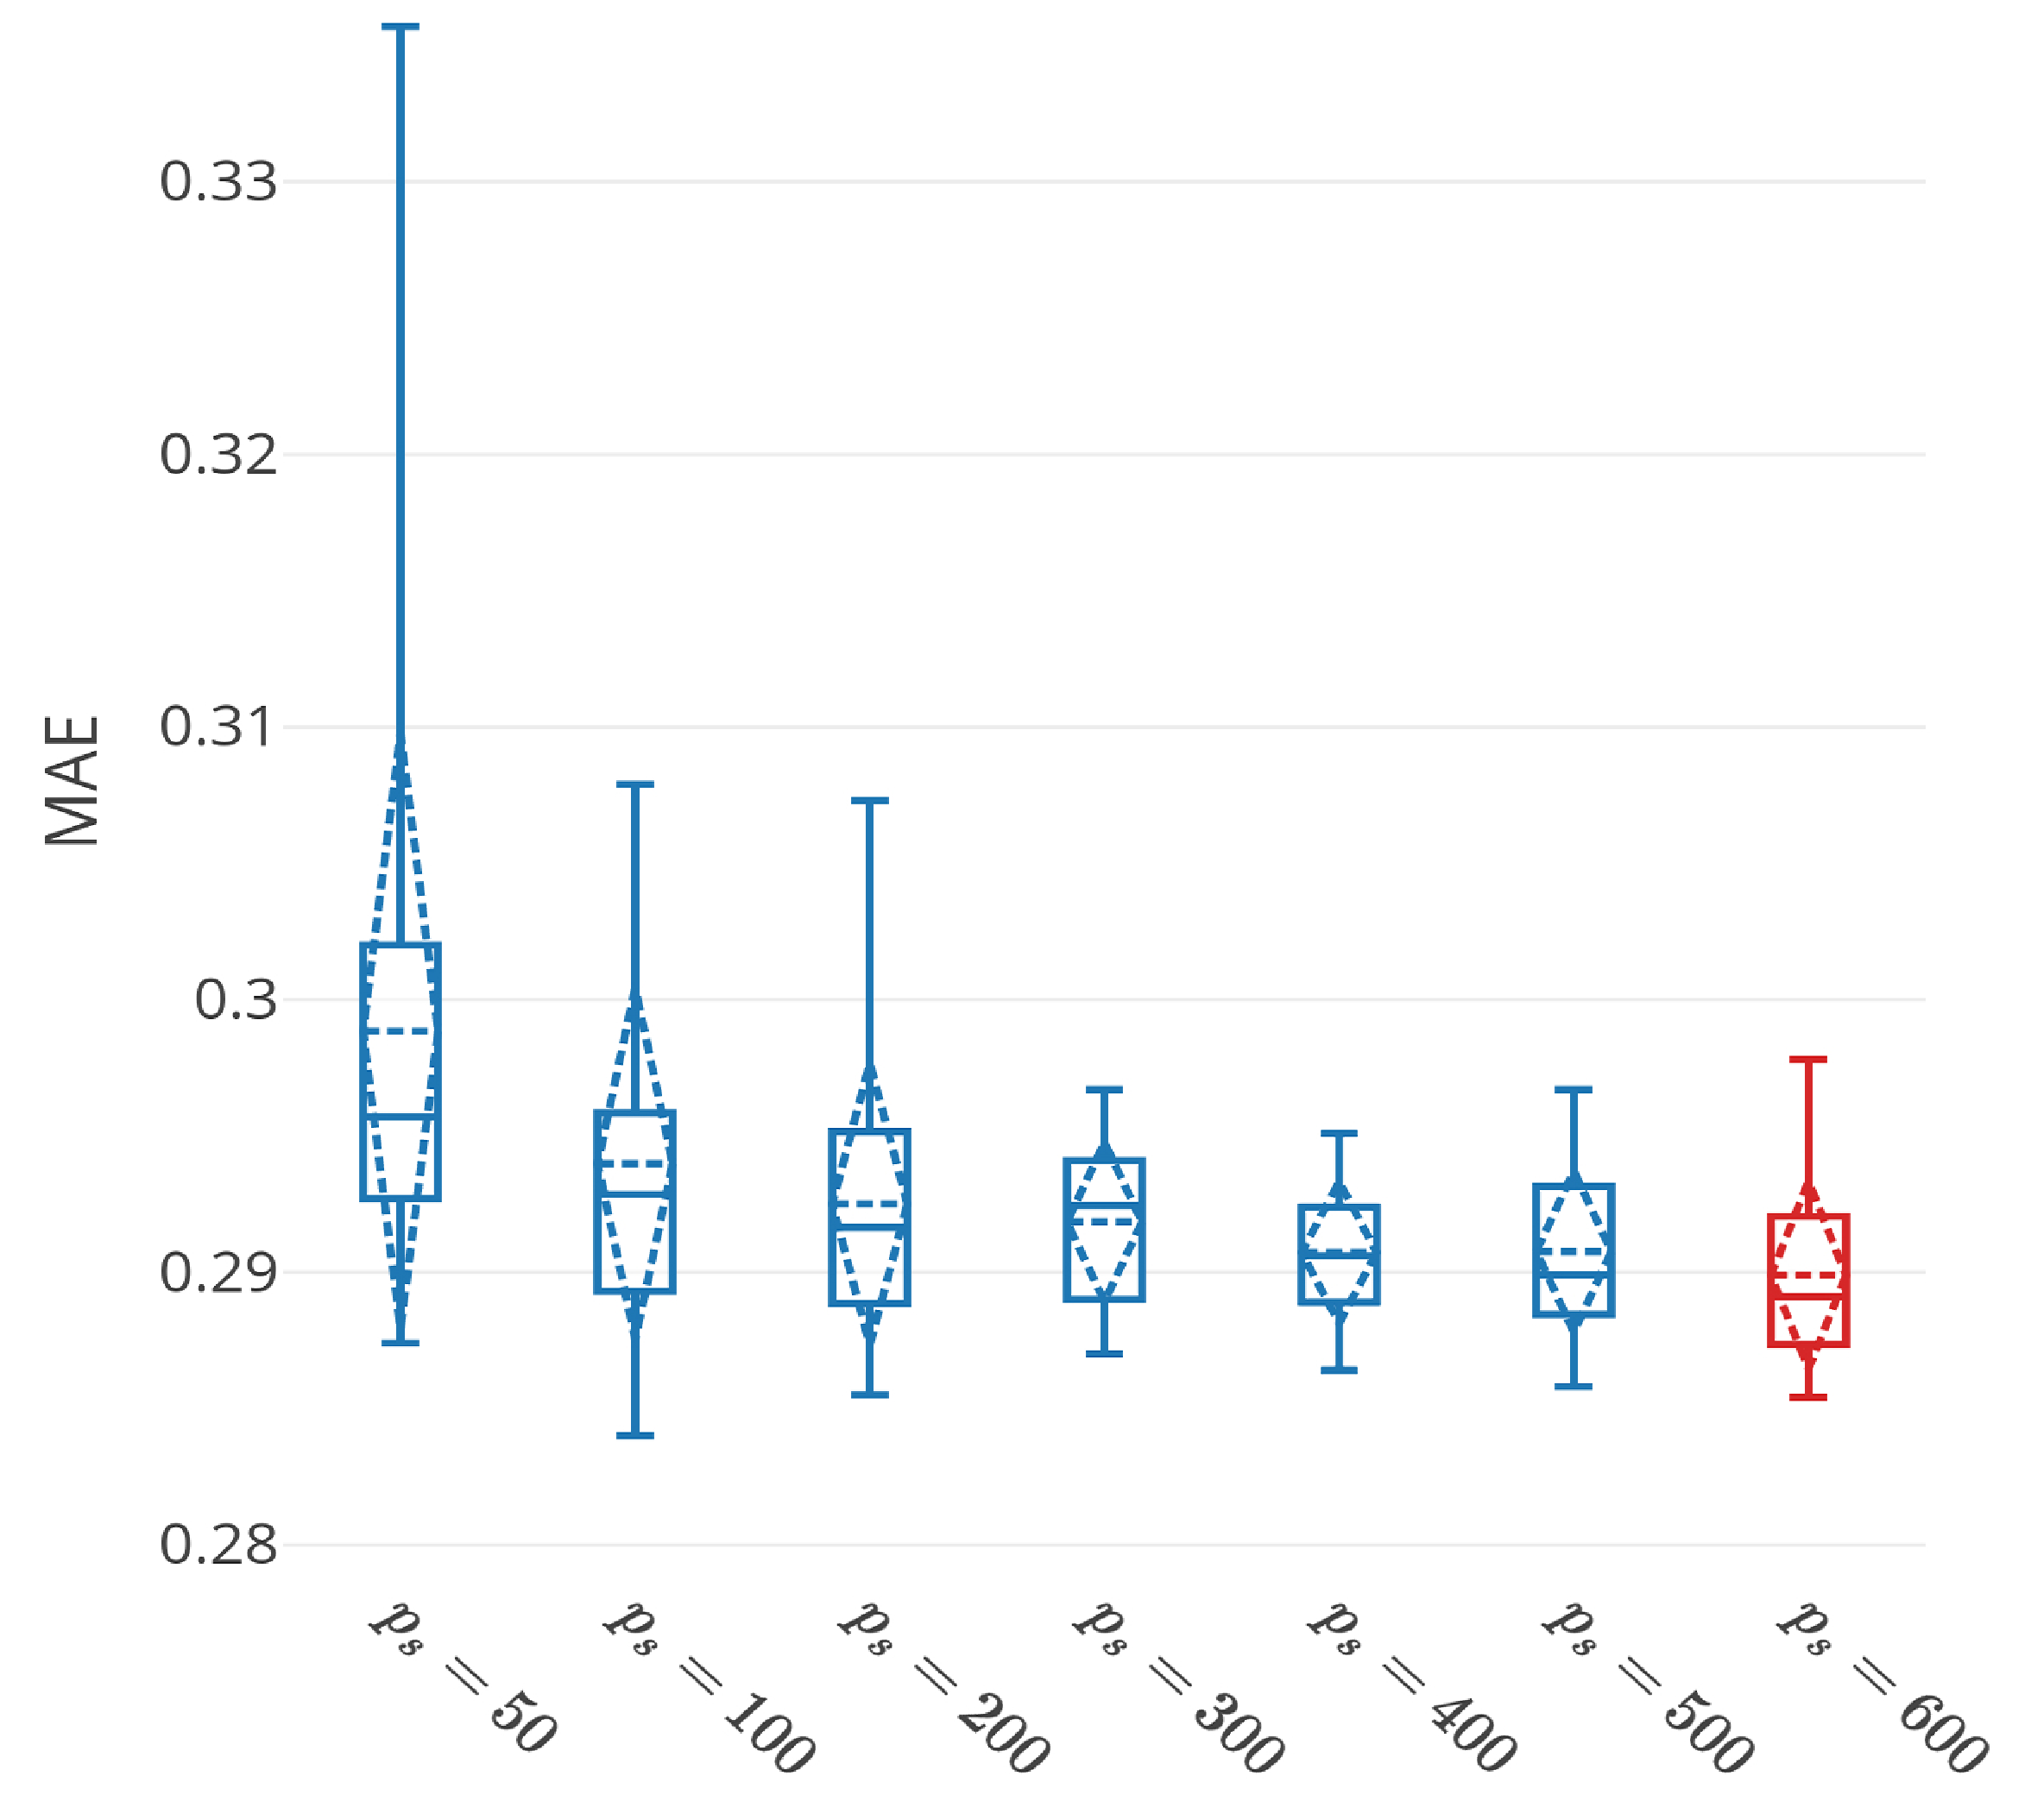
\includegraphics[width=0.75\textwidth =0.2cm 0.2cm 0.2cm 0.2cm]{images/tn2_multi_cpu_best_ps_scale.pdf}
		\caption{MAE accuracy fluctuation comparison of with different population sizes} 
		\label{tn2_CPU_ps_FLGANN}
	\end{minipage}
	\hspace{0.5cm}
	\begin{minipage}[t]{8cm}
		\centering
		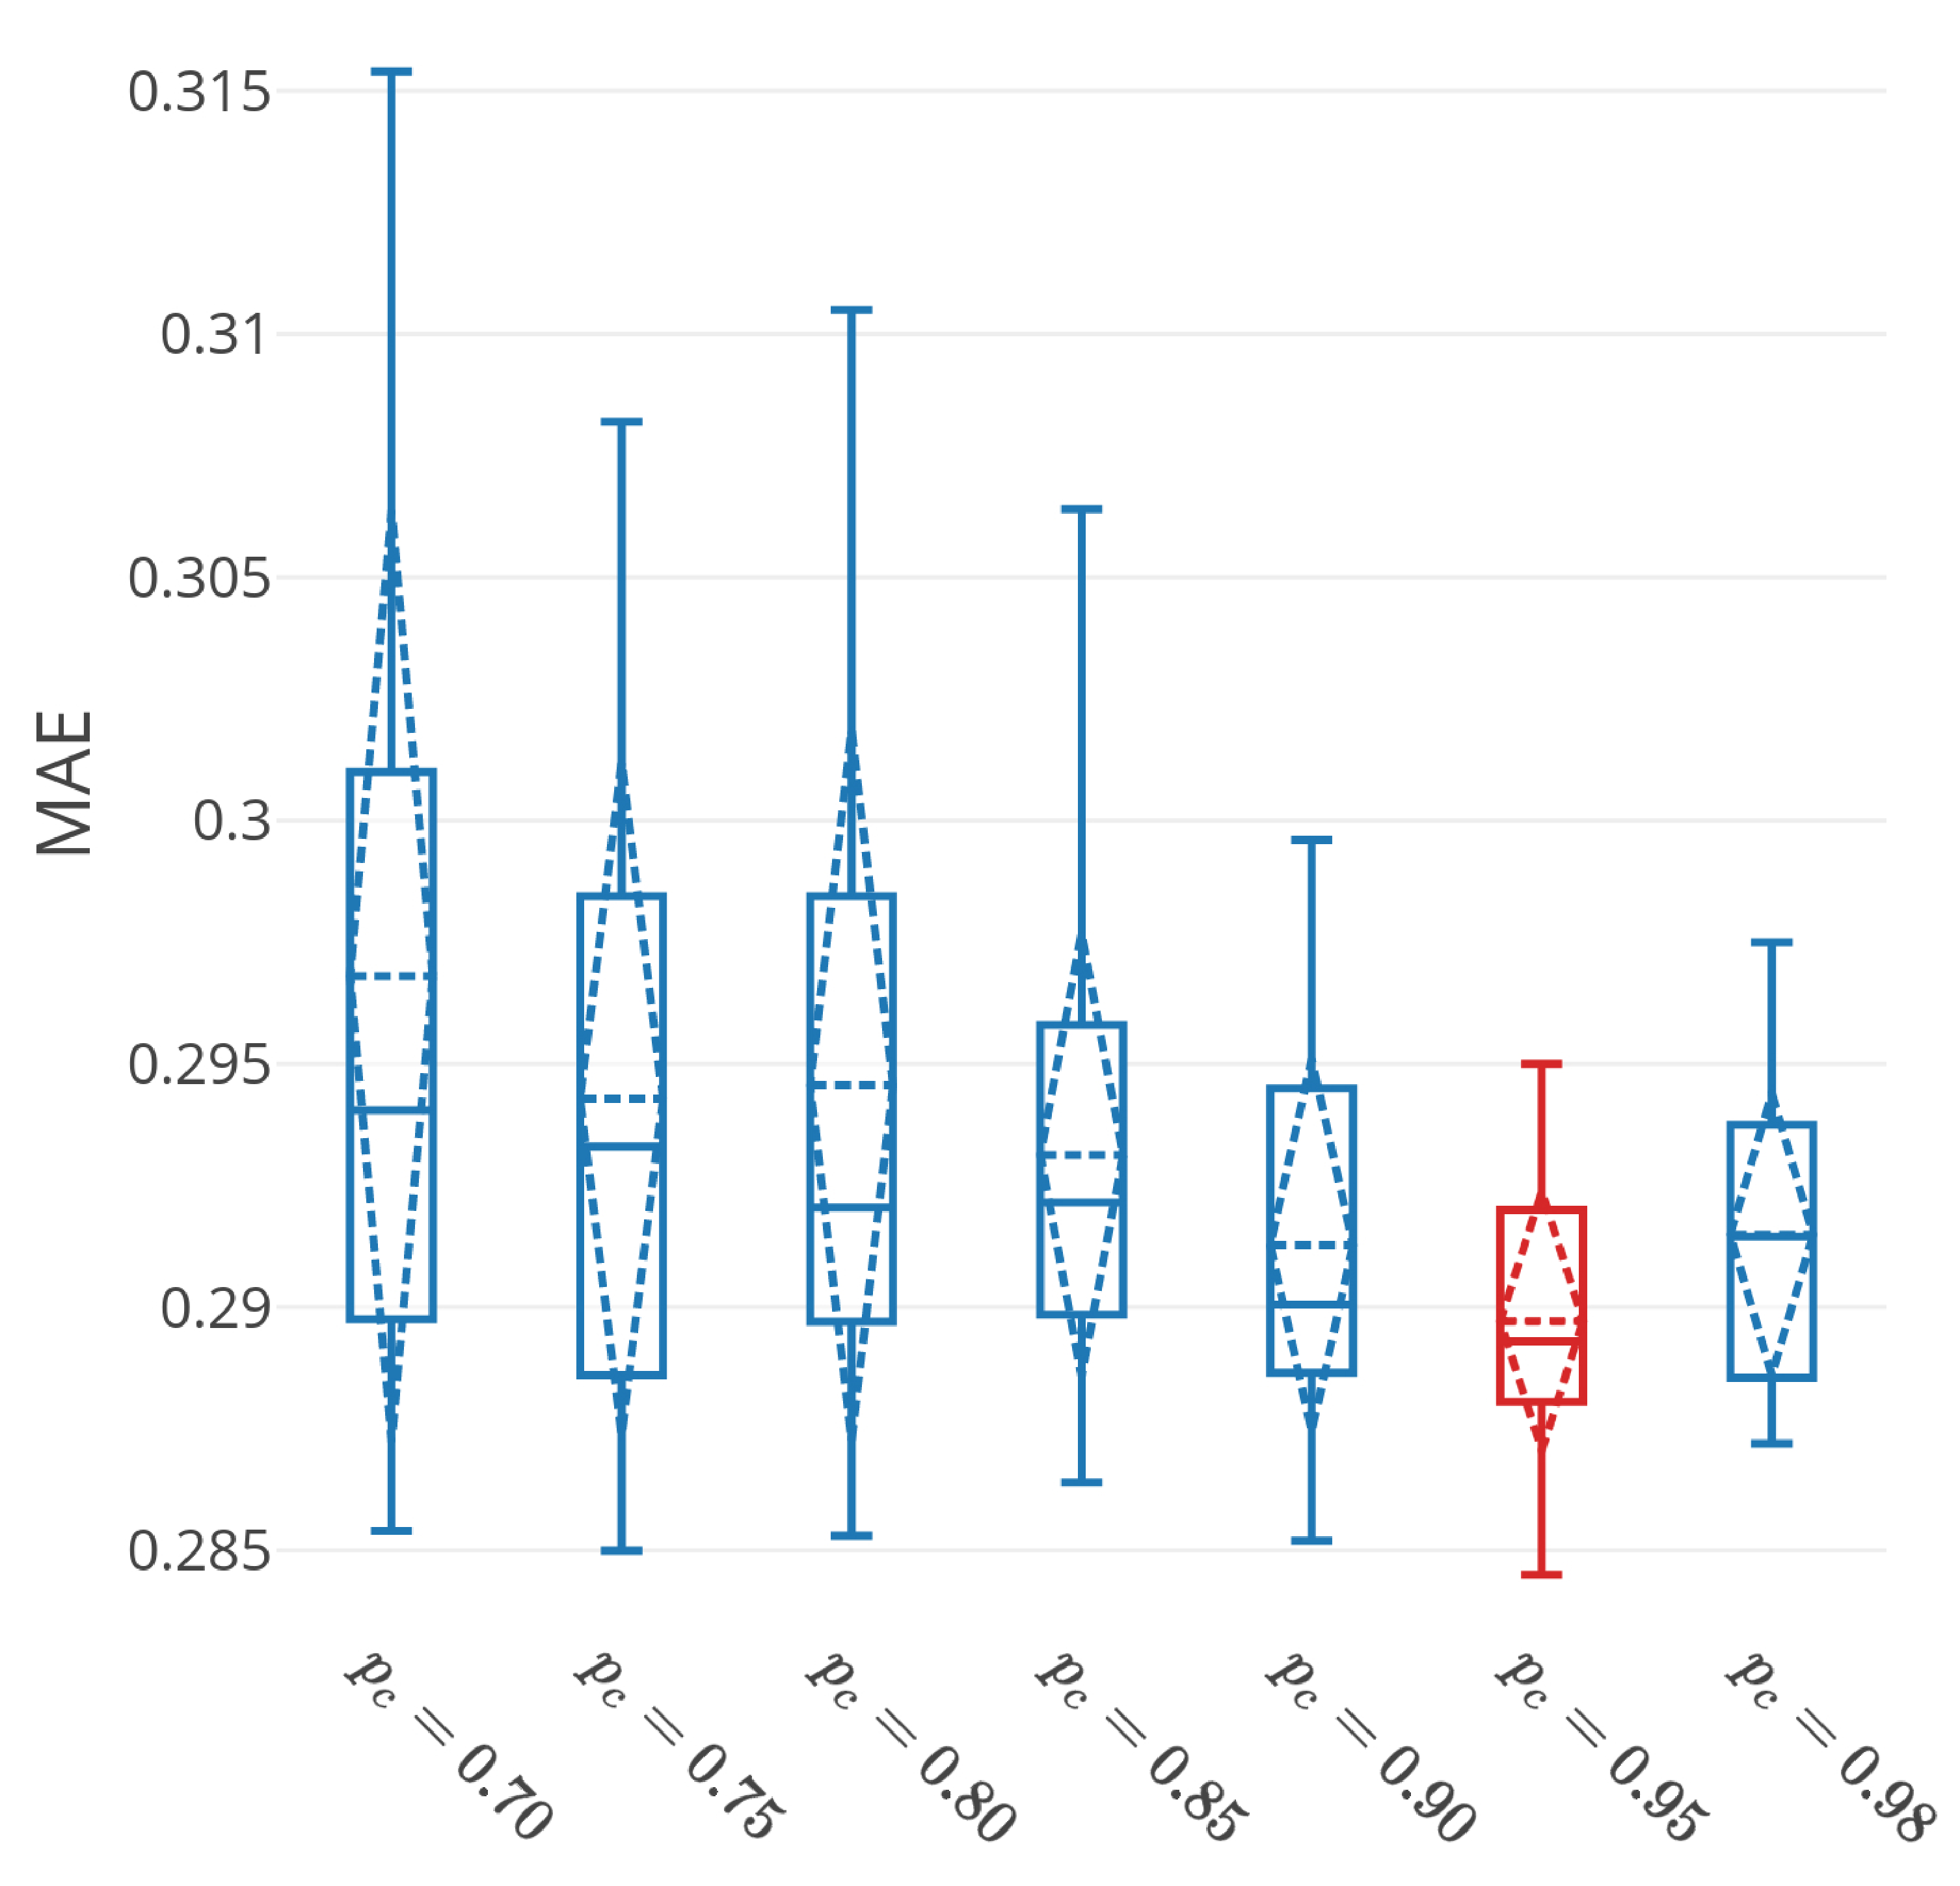
\includegraphics[width=0.75\textwidth =0.2cm 0.2cm 0.2cm 0.2cm]{images/tn2_multi_cpu_best_pc.pdf}
		\caption{MAE accuracy fluctuation comparison with different probability of two individuals exchanging crossovers} 
		\label{tn2_CPU_pc_FLGANN}
	\end{minipage}
\end{figure*}

\begin{figure*}[h]
	\centering
	\begin{minipage}[t]{8cm}
		\centering
		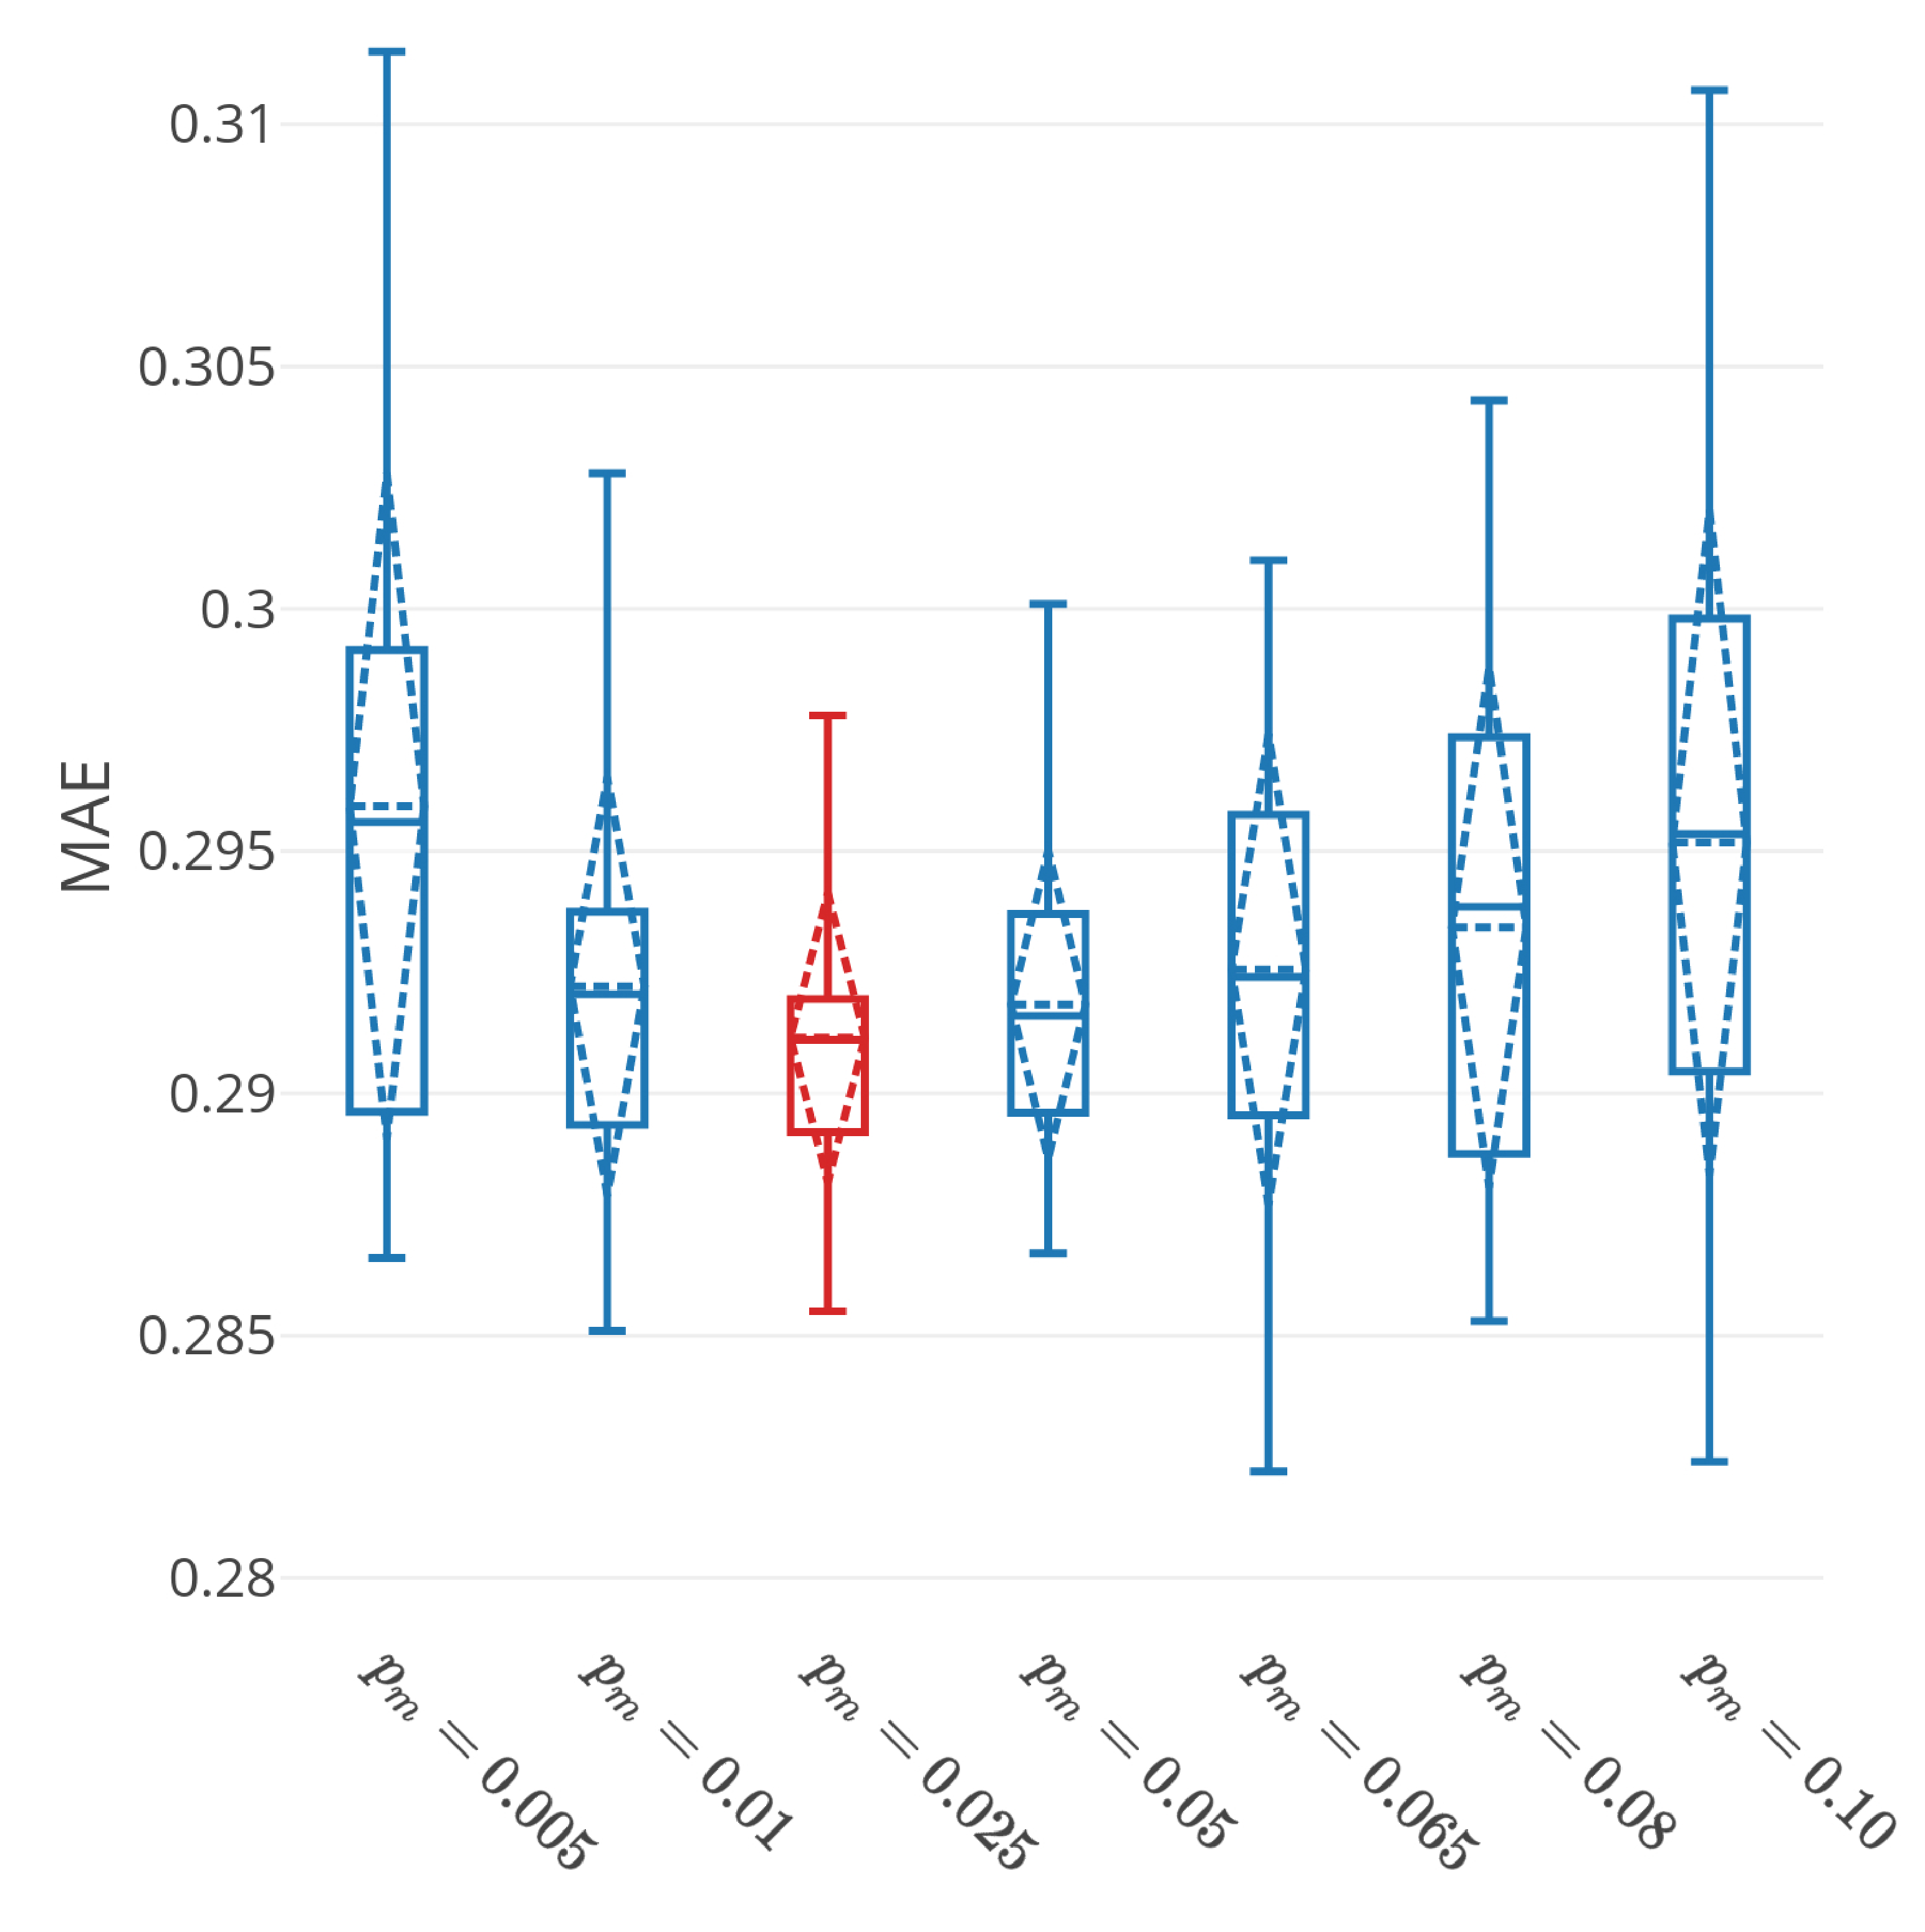
\includegraphics[width=0.75\textwidth =0.2cm 0.2cm 0.2cm 0.2cm]{images/tn2_multi_cpu_best_pm.pdf}
		\caption{MAE accuracy fluctuation comparison with different probability of individual mutation }
		\label{tn2_CPU_pm_FLGANN}
	\end{minipage}
	\hspace{0.5cm}
	\begin{minipage}[t]{8cm}
		\centering
		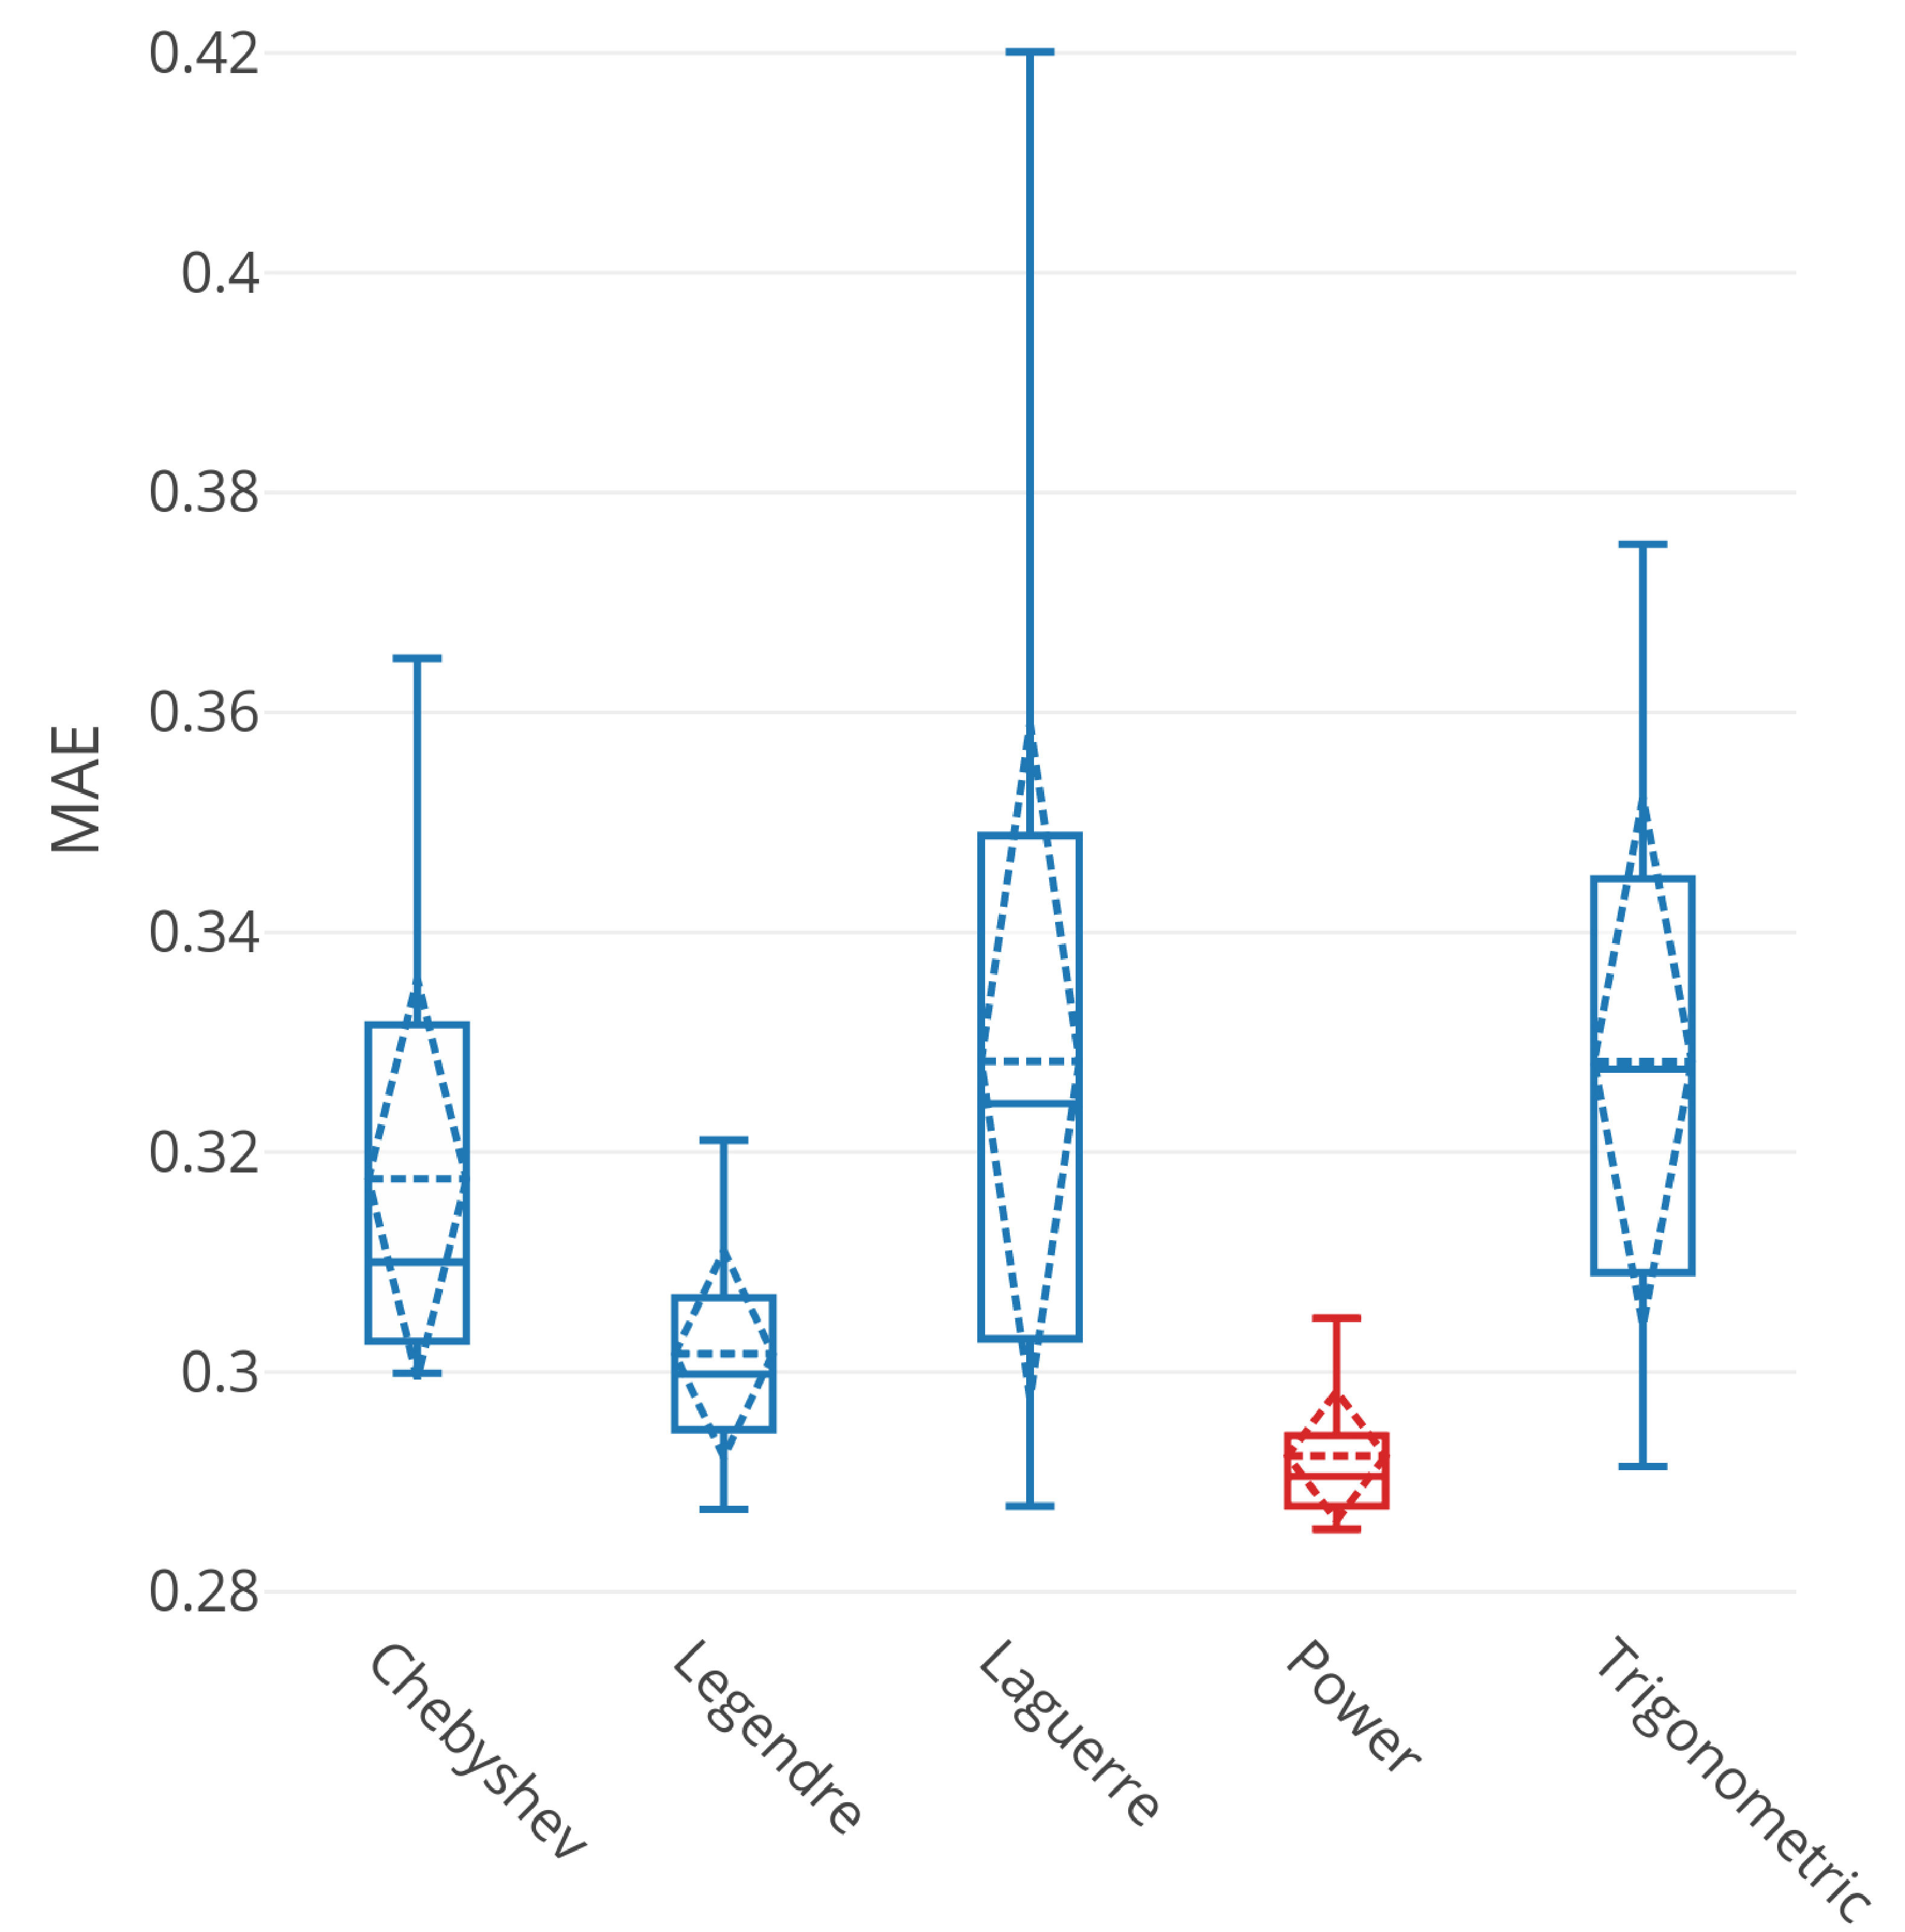
\includegraphics[width=0.75\textwidth =0.2cm 0.2cm 0.2cm 0.2cm]{images/tn2_multi_cpu_function.pdf}
		\caption{Comparison of expansion functions influence on FL-GANN}
		\label{tn3_CPU_function_FLGANN}
	\end{minipage}
\end{figure*}

\textbf{Probability of two individual exchanging crossover changing experiment.} For this test, we change $p_c$ from 0.7 to 0.98 to evaluate error accuracy via MAE and RMSE measures. Table~\ref{table:probability_crossovers} gives the average accuracy values of the measurements after 20 running times with each $p_c$. An observation can be made from those outcomes. When $p_c$ = 0.95, average MAE accuracy gets 0.2897, which is minimum value as compared to others. The better $p_c$ range for FL-GANN is 0.9 to 0.98. This means the probability of two individual exchanging crossovers to create offspring gets higher value, the results may get better. More specifically, figure~\ref{tn2_CPU_pc_FLGANN} presents the achieved MAE ranges with diverse $p_c$. Through the figure, it can conclude that the probability of two individual exchanging crossover in the range of [0.9, 0.98] producing acceptable results for the tested data.

\begin{table}[h]
\caption{Comparison of average MAE and RMSE with different probability of two individuals exchanging crossovers} 
\begin{center}
\begin{tabular}{| c | c| c |}
\hline
\textbf{Crossover Probability} & \multicolumn{2}{c|}{\textbf{Error Accuracy}}  \\ \cline{2-3} 
& MAE & RMSE \\ [0.5ex] \hline
$p_c$ = 0.70	& 0.2968	& 0.4818		\\ \hline
$p_c$ = 0.75	& 0.2943	& 0.4854	\\ \hline
$p_c$ = 0.80	& 0.2946	& 0.4852	\\ \hline
$p_c$ = 0.85	& 0.2931	& 0.4858	\\ \hline
$p_c$ = 0.90	& 0.2913	& 0.4855		\\ \hline
\textbf{$p_c$ = 0.95}	& \textbf{0.2897}	& \textbf{0.4836}	\\ \hline
$p_c$ = 0.98	& 0.2915	& 0.4869	\\ \hline
\end{tabular}
\label{table:probability_crossovers}
\end{center}
\end{table}

\textbf{Probability of individual mutation changing experiment.} Table~\ref{table:probability_mutation} shows the MAE and RMSE average values obtained after 20 running times with each $p_m$. The average MAE accuracy is 0.2911 when $p_m$ = 0.025. In the case of $p_m$ value is increased to 0.08 or even higher, the average MAE and RMSE values are bigger. This proves that the higher probability of individual mutation gets, the results may worse. Figure~\ref{tn2_CPU_pm_FLGANN} is used to illustrate MAE range with different $p_m$. Via this experiment, it can remark that MAE and RMSE results which are produced by the probability of individual mutation in the range of [0.01, 0.08] is acceptable with the tested data. 

\begin{table}[h]
\caption{Comparison of average MAE and RMSE with different probability of individual mutation} 
\begin{center}
\begin{tabular}{| c | c| c |}
\hline
\textbf{Mutation Probability} & \multicolumn{2}{c|}{\textbf{Error Accuracy}}  \\ \cline{2-3} 
& MAE & RMSE \\ [0.5ex] \hline
$p_m$ = 0.005	& 0.2959	& 0.4921	\\ \hline
$p_m$ = 0.01	& 0.2922	& 0.4847	\\ \hline
\textbf{$p_m$ = 0.025}	& \textbf{0.2911}	& \textbf{0.4829}	\\ \hline
$p_m$ = 0.05	& 0.2918	& 0.4830	\\ \hline
$p_m$ = 0.065	& 0.2926	& 0.4843	\\ \hline
$p_m$ = 0.08	& 0.2938	& 0.4847	\\ \hline
$p_m$ = 0.10	& 0.2952	& 0.4868	\\ \hline
\end{tabular}
\label{table:probability_mutation}
\end{center}
\end{table}

\subsection{Influence of Expansion Functions on FL-GANN}
\label{influence2}

\begin{table}[h]
	\caption{Comparison of expansion function influence on FL-GANN} 
	\begin{center}
		\begin{tabular}{| c | c| c | c | c | c | c |}
			\hline
			\textbf{Expansion} & \multicolumn{3}{c|}{\textbf{CPU}}  & \multicolumn{3}{c|}{\textbf{RAM}}  \\ \cline{2-7} 
			\textbf{Functions} & k = 2 & k = 3 & k = 5 & k = 2 & k = 3 & k = 5 \\ [0.5ex] \hline
			Chebyshev  & 0.3208	&  0.3654	& 0.3424  & \textbf{0.0205} & 0.0244 & 0.0288  \\ \hline
			Legendre & 0.2932	& \textbf{0.2908}	  	& 0.3347  & 0.0211 & 0.0227 & \textbf{0.0211}   \\ \hline 
			Laguerre & 0.4102	& 0.4889 	& 0.4485   & 0.0283 & 0.0333 & 0.0342  \\ \hline
			Power & \textbf{0.2860}	& 0.2915	 	& \textbf{0.2914}  & 0.0215 & \textbf{0.0206} & 0.0228  \\  \hline
			Trigo$^*$ & 0.3069	& 0.3257		& 0.4388   & 0.0346 & 0.0233 & 0.0261  \\ \hline
			\multicolumn{7}{l}{$^*$Trigonometric function}
		\end{tabular}
		\label{table:changing_expansion_functions}
	\end{center}
\end{table}

The goal of this experiment is to evaluate the influence of different expansion functions on our FL-GANN in the learning phase. In this way, we test five popular expansion functions including Chebyshev, Legendre, Laguerre, Power, and Trigonometric. The input data is multivariate. The sliding window $k$ in this experiment is set to 2, 3, and 5. The gained MAE outcomes with CPU and memory are given through Table~\ref{table:changing_expansion_functions}. In which, Power Series function produces the smallest MAE values, which are 0.2860 with $k$ = 2, 0.2914 with $k$ = 5 (CPU prediction), and 0.0206 with $k$ = 3 (memory forecast). On the other hand, Legendre function brings two minimum MAE values, which are 0.2908 with $k$ = 3 (CPU prediction) and 0.0211 with $k$ = 5 (memory forecast). Unfortunately, Laguerre and Trigonometric functions do not yield any the smallest MAE in our evaluations.

In order to more objectively evaluate Power Series and Legendre functions with FL-GANN, we carry on a small additional experiment for CPU prediction with $k$ = 3. Thus, we run 20 times for each the function, obtained MAE values of these all runs are shown by the box-and-whisker diagram~\ref{tn3_CPU_function_FLGANN}. It can be conclude that MAE fluctuation of the Power Series function is the smallest, also the average MAE (intermittent line in the box) is also the smallest as compared to Legendre function. 

\section{Conclusion and future work}
\label{conclusion}
In this paper, we presented our designs for a novel cloud resource prediction system using functional-link neural network. We also proposed the use of genetic algorithm instead of back-propagation technique with gradients descent to overcome drawbacks of the training process for traditional FLNN. Besides, in our system, the multiple resource metrics are processed simultaneously using several proposed data preprocessing mechanisms. This helps the prediction system can forecast more precisely resource consumptions in advance because the metrics often have relationship each other. We tested our FL-GANN model with a real dataset provided by Google. The achieved results show that although the forecast method is simple but it can bring good performance in prediction process even though the system exploits multivariate data. The outcomes also prove our proposals can be applied to practice. In the near future, we plan to evaluate several other variants of FLNN and to develop an auto-scaler service with decision phase for clouds using this prediction technique.

\section*{Acknowledgment} This research is supported by
the Vietnamese MOETs project No. B2017-BKA-32 Research on developing software framework to integrate IoT gateways for fog computing deployed on multi-cloud environment,
VEGA 2/0167/16 Methods and algorithms for the semantic processing of Big Data in distributed computing environment, and
APVV-17-0619 Urgent Computing for Exascale Data (U-COMP).

%\section*{Acknowledgment}
%
%The preferred spelling of the word ``acknowledgment'' in America is without 
%an ``e'' after the ``g''. Avoid the stilted expression ``one of us (R. B. 
%G.) thanks $\ldots$''. Instead, try ``R. B. G. thanks$\ldots$''. Put sponsor 
%acknowledgments in the unnumbered footnote on the first page.

%\section*{References}
%
%Please number citations consecutively within brackets \cite{b1}. The 
%sentence punctuation follows the bracket \cite{b2}. Refer simply to the reference 
%number, as in \cite{b3}---do not use ``Ref. \cite{b3}'' or ``reference \cite{b3}'' except at 
%the beginning of a sentence: ``Reference \cite{b3} was the first $\ldots$''
%
%Number footnotes separately in superscripts. Place the actual footnote at 
%the bottom of the column in which it was cited. Do not put footnotes in the 
%abstract or reference list. Use letters for table footnotes.
%
%Unless there are six authors or more give all authors' names; do not use 
%``et al.''. Papers that have not been published, even if they have been 
%submitted for publication, should be cited as ``unpublished'' \cite{b4}. Papers 
%that have been accepted for publication should be cited as ``in press'' \cite{b5}. 
%Capitalize only the first word in a paper title, except for proper nouns and 
%element symbols.


\begin{thebibliography}{00}

\bibitem{ref_hipel}
Hipel, Keith W., and A. Ian McLeod. Time series modelling of water resources and environmental systems. Vol. 45. Elsevier, 1994.

\bibitem{ref_pao}
Pao, Yohhan. "Adaptive pattern recognition and neural networks." (1989).

\bibitem{ref_majhi}
Majhi, Ritanjali, Ganapati Panda, and Gadadhar Sahoo. "Development and performance evaluation of FLANN based model for forecasting of stock markets." Expert systems with Applications 36.3 (2009): 6800-6808.

\bibitem{ref_rout}
Majhi, Babita, Minakhi Rout, Ritanjali Majhi, Ganapati Panda, and Peter J. Fleming. "New robust forecasting models for exchange rates prediction." Expert Systems with Applications 39, no. 16 (2012): 12658-12670.

\bibitem{ref_khan}
Khandelwal, Ina, Udit Satija, and Ratnadip Adhikari. "Forecasting seasonal time series with functional link artificial neural network." Signal Processing and Integrated Networks (SPIN), 2015 2nd International Conference on. IEEE, 2015.

\bibitem{ref_sahoo}
Sahoo, Deepti Moyi, and Snehashish Chakraverty. "Functional link neural network learning for response prediction of tall shear buildings with respect to earthquake data." IEEE Transactions on Systems, Man, and Cybernetics: Systems 48.1 (2018): 1-10.

\bibitem{ref_dehuri}
Dehuri, Satchidananda, and Sung-Bae Cho. "A comprehensive survey on functional link neural networks and an adaptive PSO–BP learning for CFLNN." Neural Computing and Applications 19.2 (2010): 187-205.

\bibitem{ref_motana}
Montana, David J., and Lawrence Davis. "Training Feedforward Neural Networks Using Genetic Algorithms." IJCAI. Vol. 89. 1989.

\bibitem{ref_dang}
Tran, D., Tran, N., Nguyen, G., and Nguyen, B. M. (2017). A proactive cloud scaling model based on fuzzy time series and SLA awareness. Procedia Computer Science, 108, 365-374.

\bibitem{ref_nhuan} 
Tran, N., Nguyen, T., Nguyen, B. M., and Nguyen, G.. A Multivariate Fuzzy Time Series Resource Forecast Model for Clouds using LSTM and Data Correlation Analysis. In Procedia Computer Science, Elsevier, 22nd International Conference on Knowledge-Based and Intelligent Information $\&$ Engineering Systems (KES), Belgrade, 2018, in press.

\bibitem{ref_blanco}
Blanco, Armando, Miguel Delgado, and Maria C. Pegalajar. "A real-coded genetic algorithm for training recurrent neural networks." Neural networks 14.1 (2001): 93-105.

\bibitem{ref_dehuri_2}
Dehuri, Satchidananda, Bijan Bihari Mishra, and Sung-Bae Cho. "Genetic feature selection for optimal functional link artificial neural network in classification." International Conference on Intelligent Data Engineering and Automated Learning. Springer, Berlin, Heidelberg, 2008.

\bibitem{ref_google_trace}
Reiss, Charles, et al. "Heterogeneity and dynamicity of clouds at scale: Google trace analysis." Proceedings of the Third ACM Symposium on Cloud Computing. ACM, 2012.

\bibitem{ref_prevost}
Prevost, J. J., Nagothu, K., Kelley, B., $\&$ Jamshidi, M. (2011, June). Prediction of cloud data center networks loads using stochastic and neural models. In System of Systems Engineering (SoSE), 2011 6th International Conference on (pp. 276-281). IEEE.

\end{thebibliography}

\end{document}
